% TO-DO:

\input{../YKY-preamble.tex}

\usepackage{color}
\usepackage{mathtools}
\usepackage{hyperref}

%\setsansfont{Latin Modern Sans}
%\renewcommand{\familydefault}{\sfdefault}

%\usepackage[backend=biber,style=numeric]{biblatex}
%\bibliography{../AGI-book}
% \renewcommand*{\bibfont}{\footnotesize}

\usepackage{graphicx} % Allows including images
\usepackage{tikz-cd}
\usepackage{tikz}
\usepackage[export]{adjustbox}% http://ctan.org/pkg/adjustbox
\usepackage{verbatim} % for comments

% \numberwithin{equation}{subsection}

\newcommand{\underdash}[1]{%
	\tikz[baseline=(toUnderline.base)]{
		\node[inner sep=1pt,outer sep=10pt] (toUnderline) {#1};
		\draw[dashed] ([yshift=-0pt]toUnderline.south west) -- ([yshift=-0pt]toUnderline.south east);
	}%
}%

\DeclareSymbolFont{symbolsC}{U}{txsyc}{m}{n}
\DeclareMathSymbol{\strictif}{\mathrel}{symbolsC}{74}

\newcommand{\highlight}[1]{\colorbox{pink}{$\displaystyle #1$}}

\newcommand{\emp}[1]{{\color{violet}\textbf{#1}}}
\newcommand*\confoundFace{$\vcenter{\hbox{\includegraphics[scale=0.2]{../confounded-face.jpg}}}$}

\newcommand{\witness}{\scalebox{0.6}{$\blacksquare$}}
% \newcommand{\Heytingarrow}{\mathrel{-}\mathrel{\triangleright}}
\providecommand\Heytingarrow{\relbar\joinrel\mathrel{\vcenter{\hbox{\scalebox{0.75}{$\rhd$}}}}}

\makeatletter
\newcommand{\verbatimfont}[1]{\def\verbatim@font{#1}}%
\makeatother
\verbatimfont{\rmfamily}

\begin{document}

\title{\cc{\bfseries\color{blue}{\Huge White paper}}
{{\Huge White paper}}}
% \author{YKY} % Your name
%\institute[] % Your institution as it will appear on the bottom of every slide, may be shorthand to save space
%{
%Independent researcher, Hong Kong \\ % Your institution for the title page
%\medskip
%\textit{generic.intelligence@gmail.com} % Your email address
%}
% \date{\today} % Date, can be changed to a custom date

% \maketitle
\date{\vspace*{-2cm} \today}
\maketitle

% \section{Introduction}


This is the original Transformer architecture:
\begin{equation}
\vcenter{\hbox{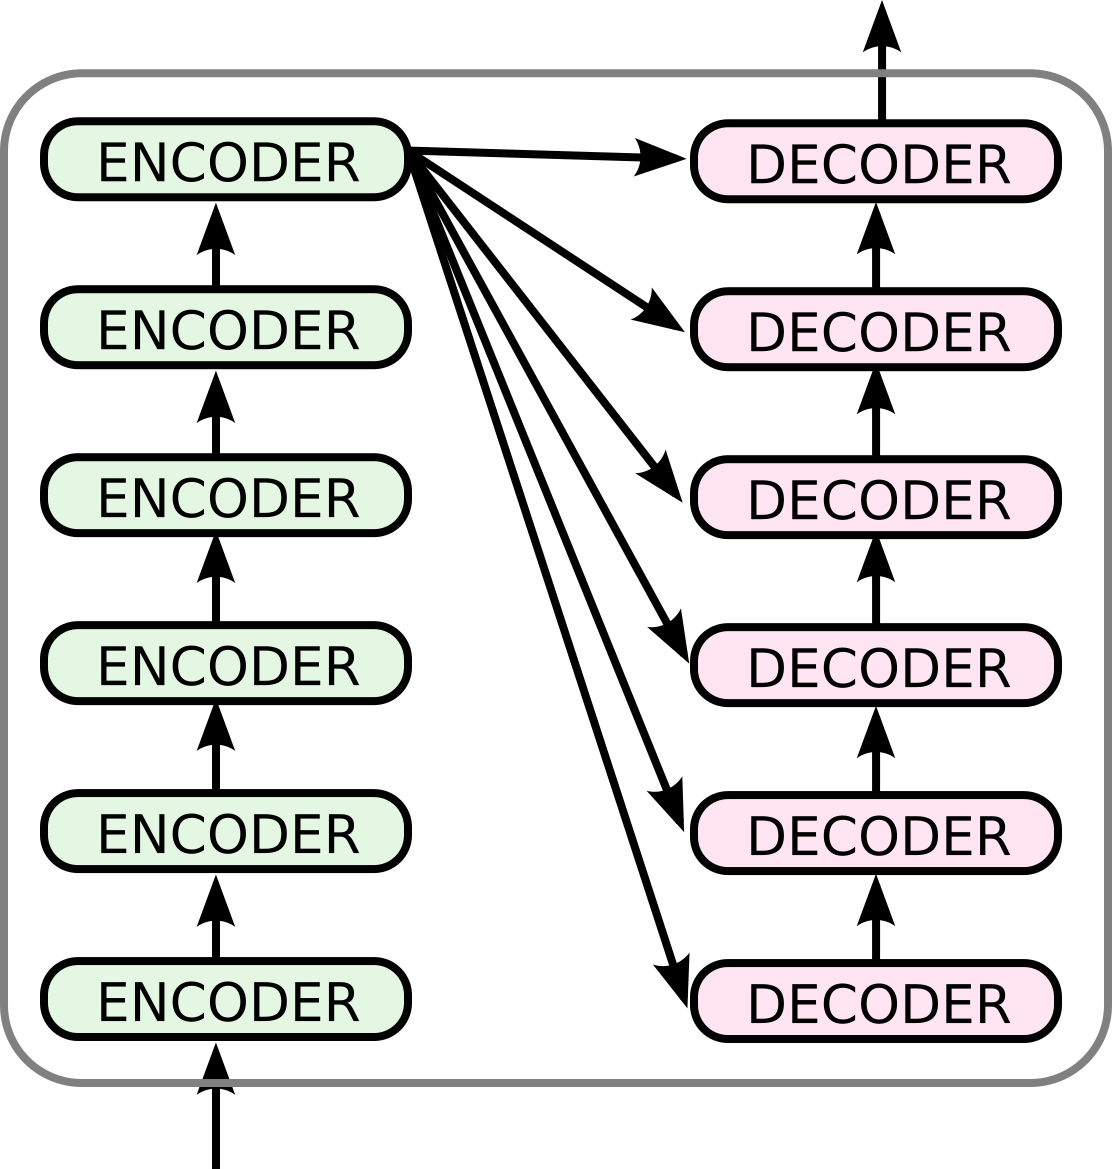
\includegraphics[scale=0.7]{original-BERT-Transformer.png}}}
\end{equation}

This is the ``Encoder'' part:
\begin{equation}
\vcenter{\hbox{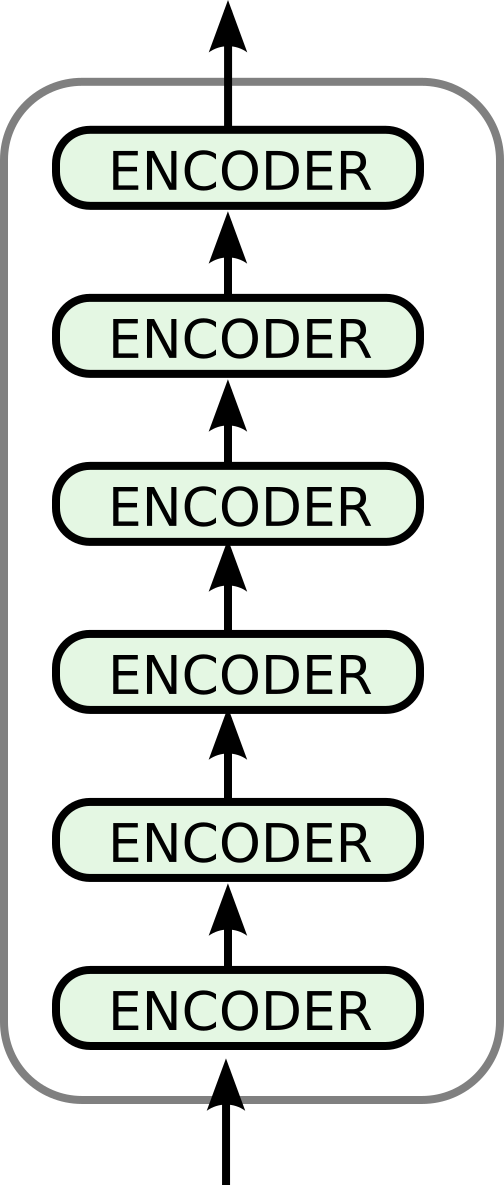
\includegraphics[scale=0.7]{original-BERT-encoder.png}}}
\end{equation}
(A friend told me that BERT only uses the Encoder part of Transformer.)

% We may regard the intermediate result between the encoder and decoder as the ``hidden state'' of BERT, 反正它是 一步就 go through 的。

所不同的是,在 强化学习里,狀態 is iteratively updated:
\begin{equation}
\vcenter{\hbox{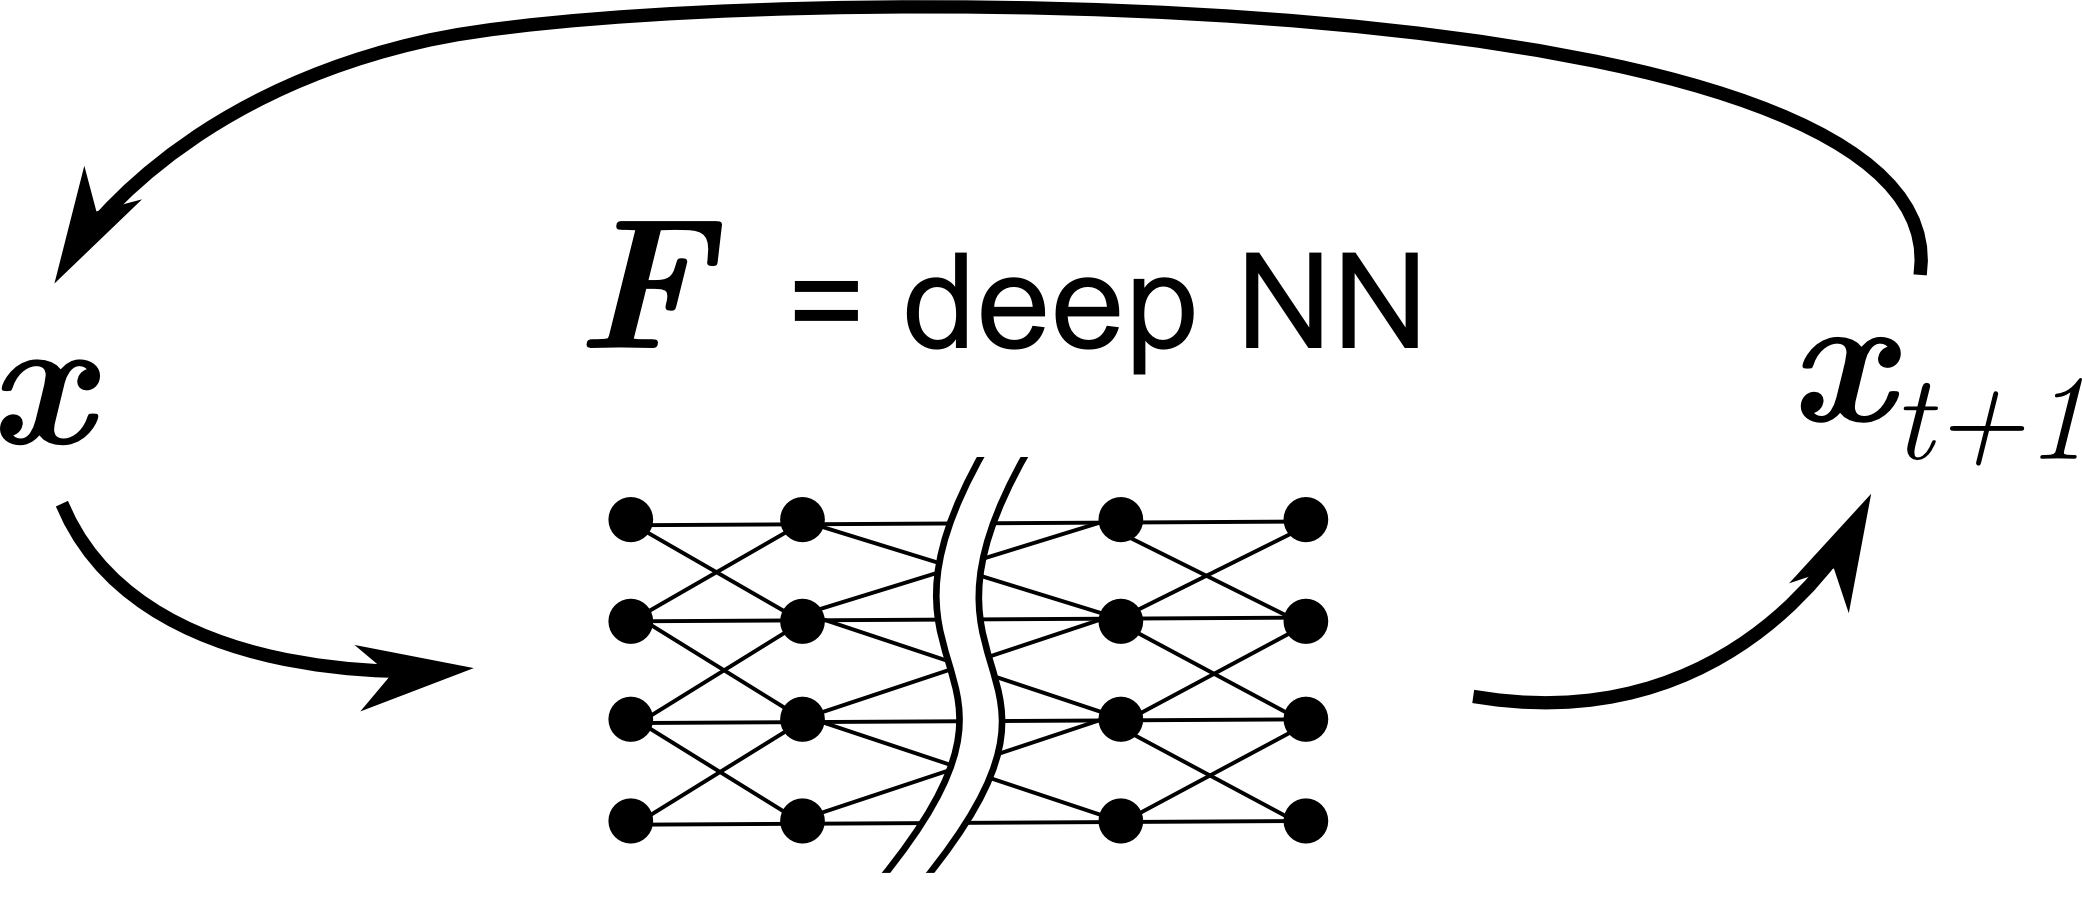
\includegraphics[scale=0.9]{../2019/genifer-model-00.png}}}
\end{equation}

其中,input/output are reserved parts inside the state vector:
\begin{equation}
\vcenter{\hbox{\includegraphics[scale=0.7]{../2019/minimal-architecture.png}}}
\end{equation}

现在问题是我们想用 reinforcement learning 的架构,加到 BERT 上。 

首先看看 BERT 是怎样训练的:
\begin{equation}
\vcenter{\hbox{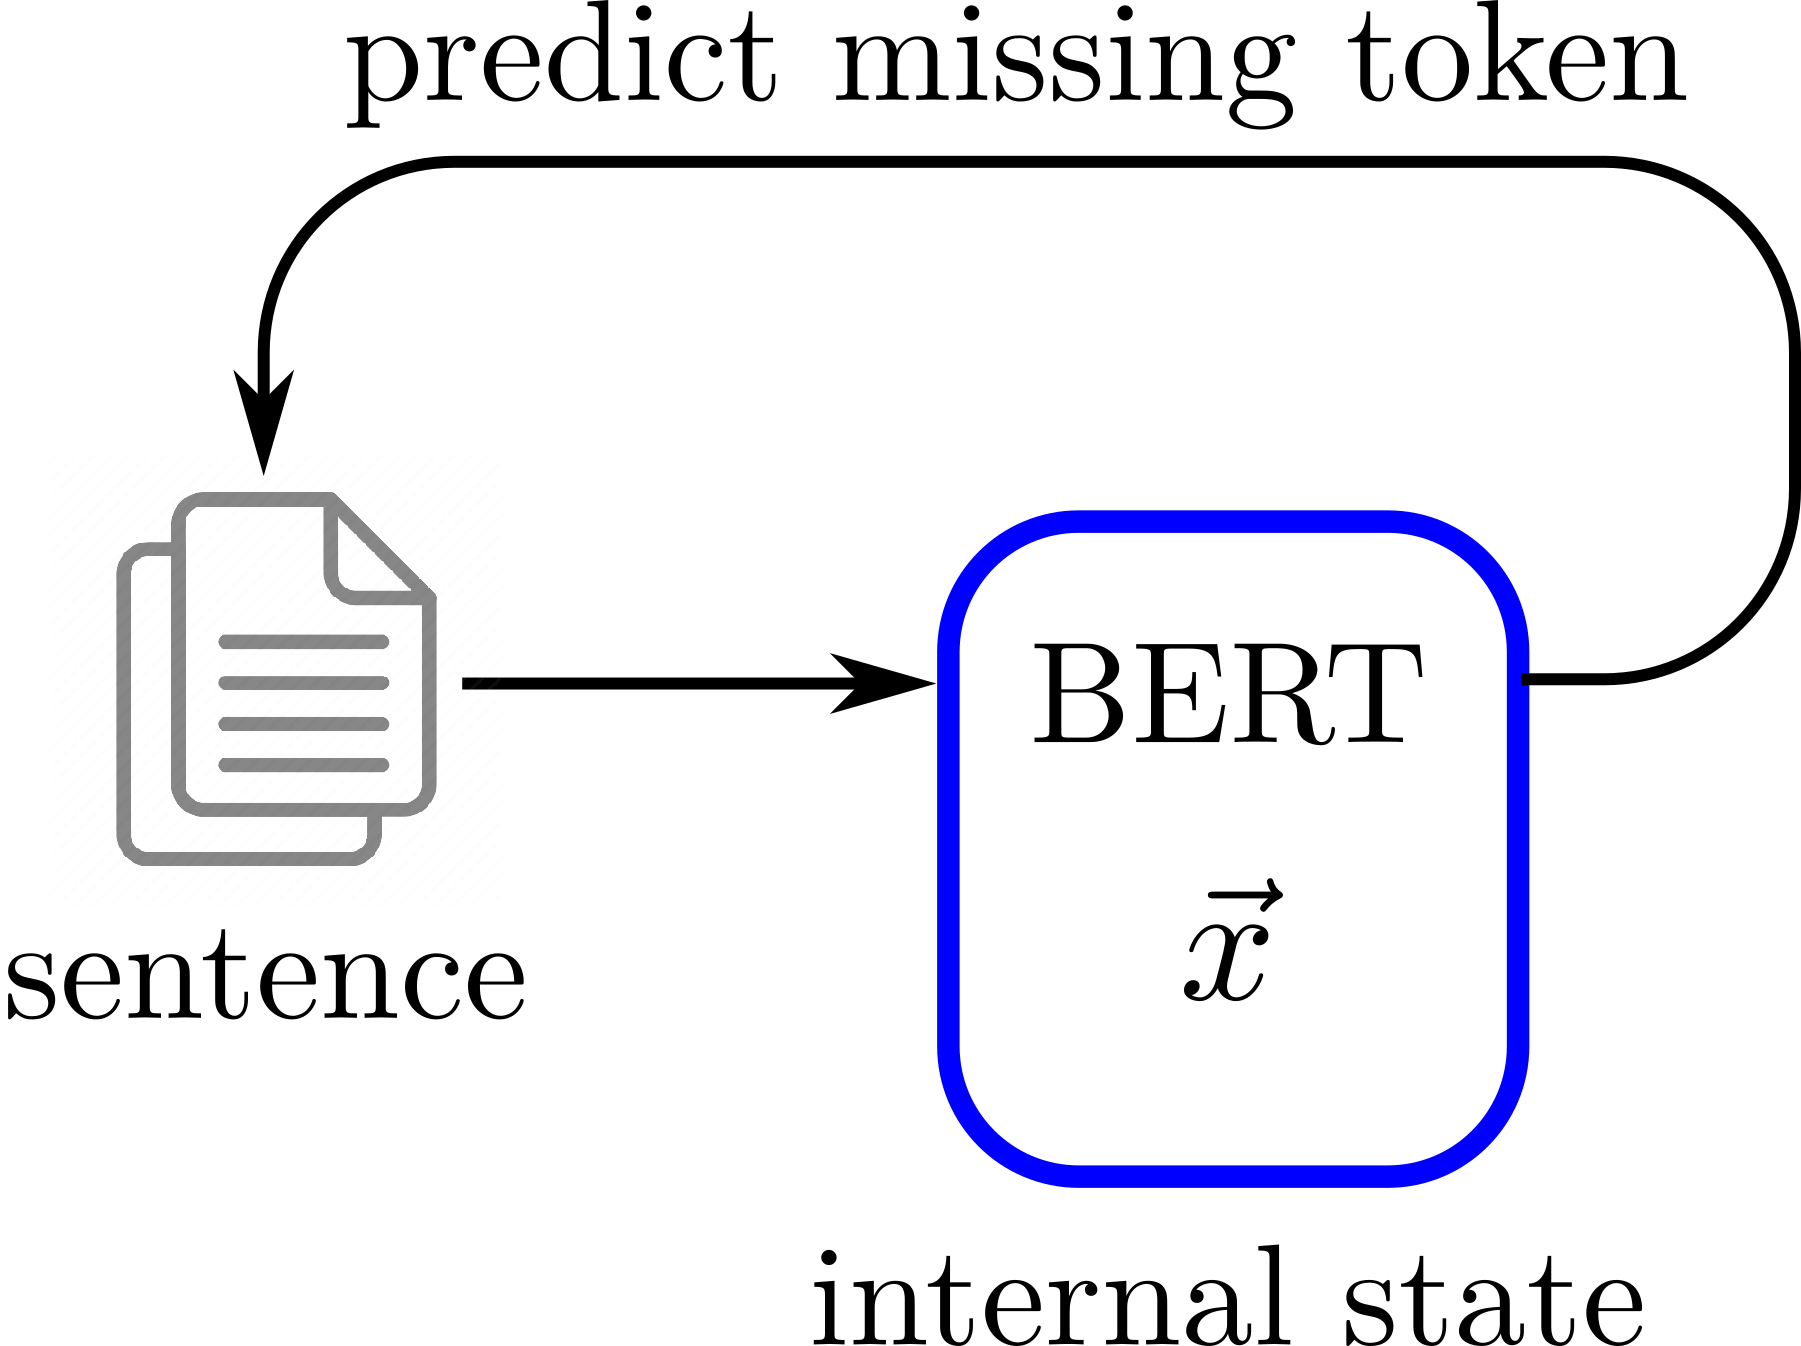
\includegraphics[scale=0.8]{BERT-training.png}}}
\end{equation}
% 注意: 在 BERT 内部其实也好像有 RNN 迴路({\color{red}红色 loop}).

%(其实我也没有详细看过 BERT 的代码,我的理解可能有误,但我和一些熟悉 BERT 的人谈过)

其实我也不太清楚怎样将 BERT 与 RL 结合,其中一篇論文是 \textbf{KG-A2C} (Knowledge-Graph Advantage Actor-Critic): \\
\tab \href{https://openreview.net/forum?id=B1x6w0EtwH}{https://openreview.net/forum?id=B1x6w0EtwH}

According to the paper, the update is done via an Advantage function $A$:
\begin{equation}
A(\vect{x}_t, a_t) = Q(\vect{x}_t, a_t) - V(\vect{x}_t)
\end{equation}
\begin{equation}
Q(\vect{x}_t, a_t) = \mathbb{E} [ R_t + \gamma V(\vect{x}_{t+1})]
\end{equation}
where $R$ is the reward.  $V$ is the value function and $Q$ is the value function restricted to action $a$, as is standard in $Q$-learning.  This part seems pretty standard for A2C.

如果不用 BERT 而用我的 symmetric neural network 方法,可能更易:

用 symmetric neural network 的话,系统的 状态 有 \textbf{逻辑命题} ({\color{red}red} \tikz\draw[red,fill=red] (0,0) circle (.5ex);) 的结构:
\begin{equation}
\vcenter{\hbox{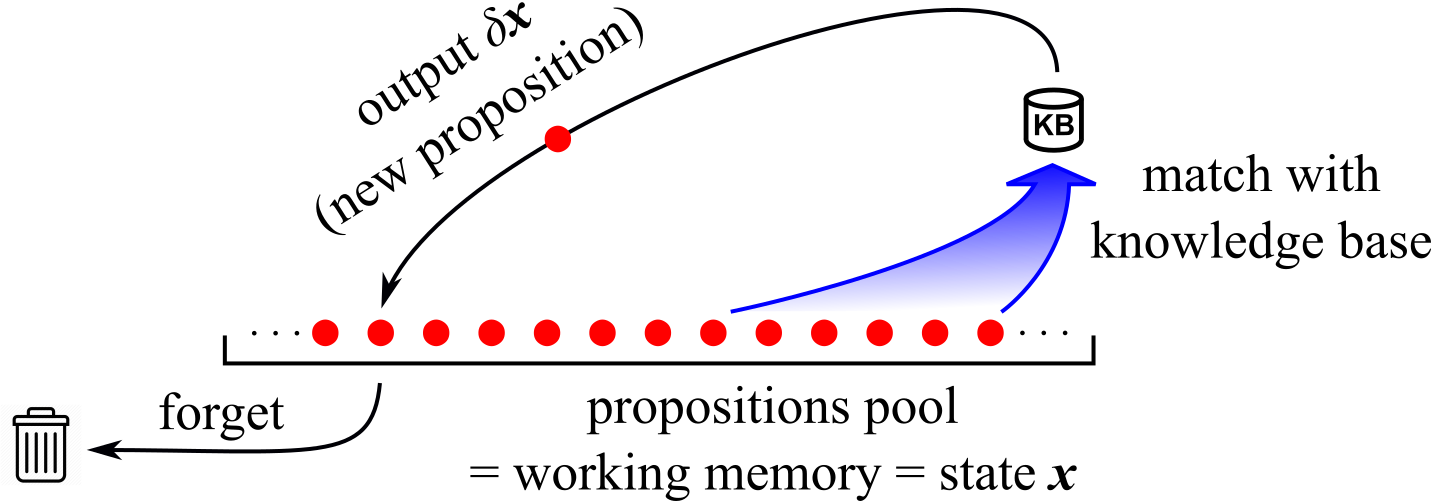
\includegraphics[scale=0.8]{../2019/classical-AI-architecture.png}}}
\end{equation}
在每个时间点 $t$,状态 以如下方式 \textbf{update}:
\begin{equation}
\vect{x}_{t+1} = \vect{x}_t \oplus \delta \vect{x} \ominus \mbox{forget}(\vect{x}_t)
\end{equation}
暂时不会 implement forgetting mechanism, 我们只是用一个足够大的 state 装下整个 NL 句子的字(每个 NL字 用一个逻辑命题),\textbf{遗忘} 时间最早的那些 命题。

在 policy gradient 方法下 reinforcement learning 的 \textbf{update} 是:
\begin{equation}
\theta := \theta + \eta \nabla_{\theta} J(\theta)
\end{equation}
where
\begin{itemize}
	\item $\theta$ = \textbf{parameter} of the policy $\pi_{\theta}$
	\item $J$ = \textbf{value} function = $\mathbb{E}[\; R(\tau) \;]$
	\item $R(\tau)$ = total \textbf{reward} of trajectory $\tau$
\end{itemize}
where a \textbf{trajectory} is a sequence of (state, action)'s:
\begin{equation}
\tau = s_0, a_0, s_1, a_1, ... s_T, a_T.
\end{equation}
and the \textbf{policy} is a probability function:
\begin{eqnarray}
\pi_{\theta}(\tau) &=& \mbox{probability of trajectory } \tau \\
 &=& p(s_0) \pi_{\theta}(a_0|s_0) p(s_1|s_0,a_0) \cdot .... \nonumber
\end{eqnarray}

%\section*{References}
% \printbibliography

\end{document} 
